\title{SMC's Tidal Disruption as a New Dark Matter Probe with Spec-S5}

\author{Himansh Rathore}
\affil{Steward Observatory, University of Arizona}

\author{Gurtina Besla}
\affil{Steward Observatory, University of Arizona}

\author{Hayden R. Foote}
\affil{Steward Observatory, University of Arizona}

\begin{figure}
    \centering
    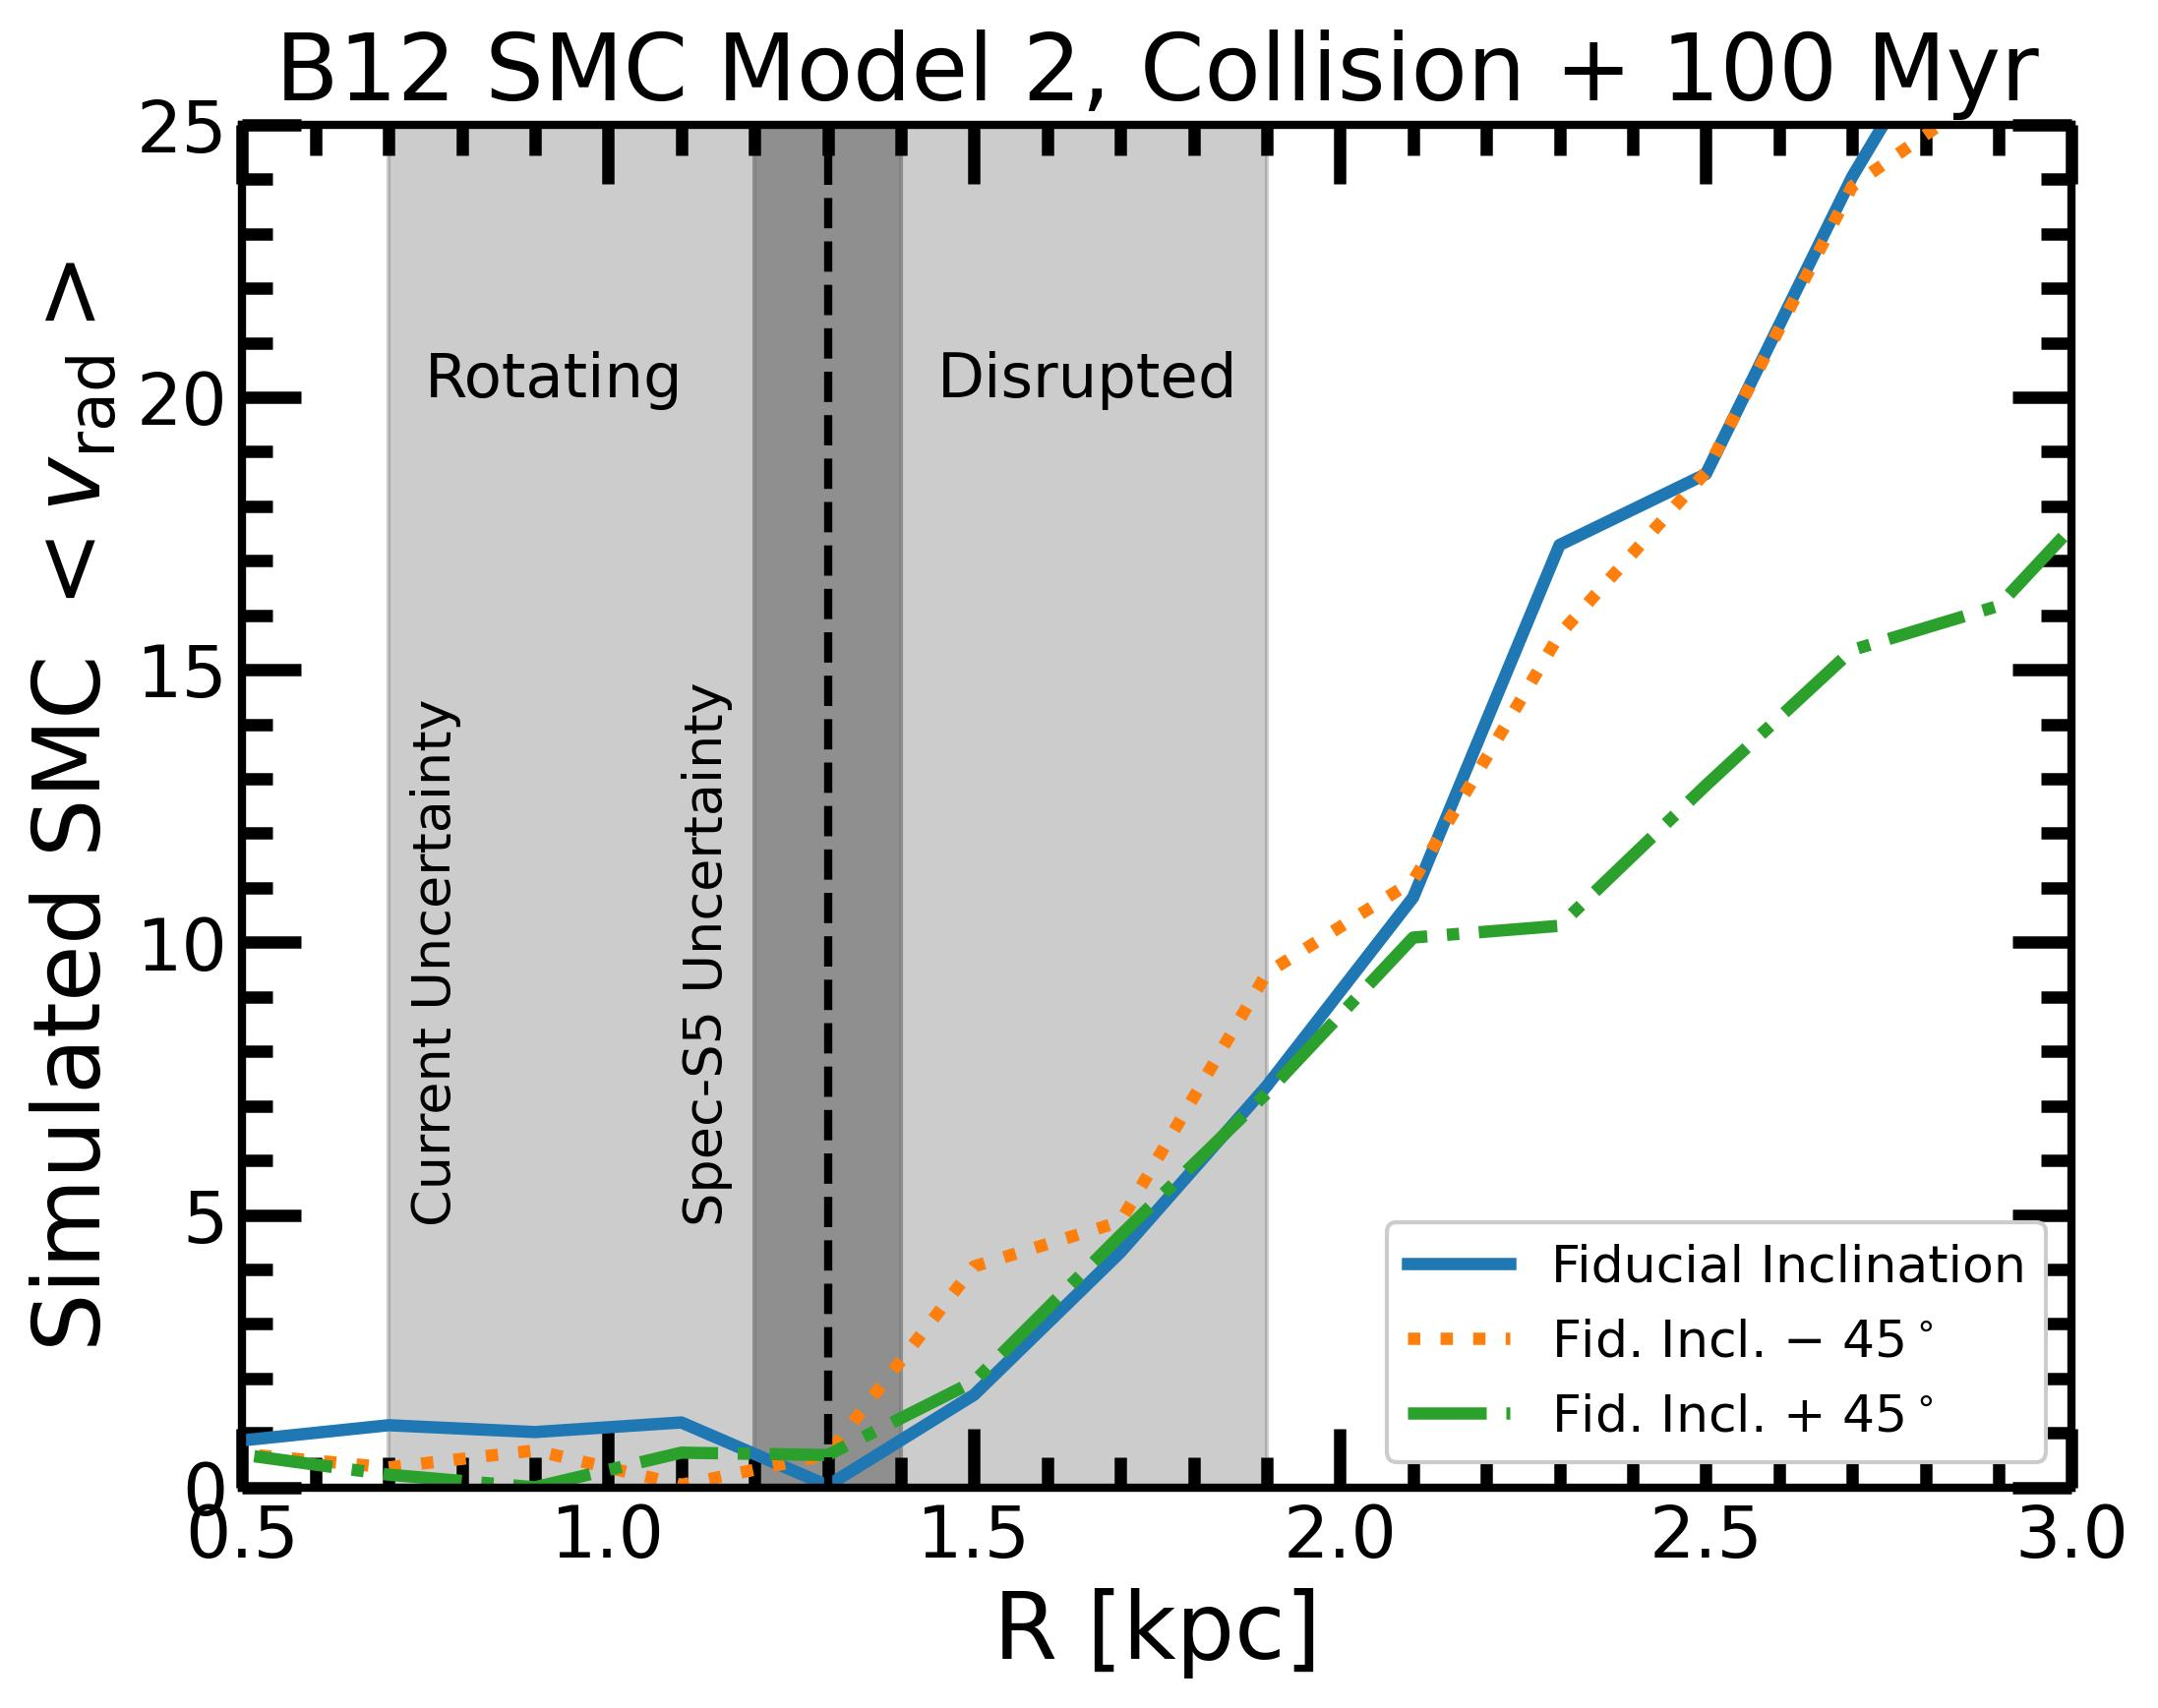
\includegraphics[width=0.5\linewidth]{vrad_prediction_specS5.jpg}
    \caption{Prediction of the SMC's tidal disruption using the B12 hydrodynamic simulations of LMC-SMC collision. The y-axis represents the azimuthally averaged line-of-sight velocity of the simulated SMC at present day (100 Myr after the collision), and the x-axis denotes the radial coordinate in the SMC. The 3 colored lines denote different on-sky inclinations assumed for the SMC. The tidal radius (1.3 kpc, vertical dashed line) separates the rotating and disrupting regions of the SMC. For $R < 1.3$ kpc, the stellar velocity field is dominated by rotation, leading to $<v_{\rm rad}> \approx 0$. For $R > 1.3$ kpc, the stellar velocity field is dominated by radially outward motions driven by the LMC's tides. The three colored lines yield the same tidal radius, indicating that the tidal radius is not sensitive to the assumed viewing perspective. Precisely constraining the observed SMC's tidal radius can yield constraints into the SMC's dark matter profile as well as interactions between dark matter particles.}
    \label{fig:smc_disruption}
\end{figure}

\textbf{Facts:} The LMC-SMC system is the nearest example of an interacting galaxy pair. In particular, the SMC has directly collided (impact parameter $\sim 2$~kpc) with the LMC $<200$~Myr ago. As such, the SMC's stellar disk is disrupting due to the LMC's gravitational tides (e.g. Zivick et al. 2021; Rathore et al. 2026).

In Figure \ref{fig:smc_disruption}, we show the present-day azimuthally averaged line-of-sight (LoS) velocity profile ($<v_{rad}>$) of the SMC in the Besla et al. 2012 (hereafter B12) hydrodynamic simulation of the LMC-SMC collision. The x-axis is separated into two regions --- "rotating" (R $< 1.3$ kpc) and "disrupting" (R $> 1.3$ kpc). The stellar velocity field at R $<1.3$ kpc is dominated by rotation, leading to a net-zero $<v_{rad}>$. The stellar velocity field at R $>1.3$ kpc is dominated by radially outward motions driven by the LMC's tides, leading to a non-zero value of $<v_{rad}>$ that increases to 15 - 30 km/s at R $= 3$ kpc. The boundary between the two regimes occurs at a radius of 1.3 kpc in the simulation, which corresponds to the SMC's tidal radius.

\textbf{Importance of Facts:} The process of tidal disruption is sensitive to the dark matter profile of the disrupting galaxy (Du et al. 2024), which in turn is sensitive to the interactions between dark matter particles (e.g. Zhang et al. 2024). As such, the SMC's tidal disruption is a new probe of dark matter physics, provided the tidal radius can be precisely constrained.

\textbf{Problem:} Precise measurements of the velocity field of the SMC's old stellar populations, like red giant stars (G $\sim 17$ mag) and red clump stars (G $\sim 20$ mag) are required to constrain the SMC's tidal radius. The measurement precision needs to be high enough that comparisons between different dark matter models is possible. In particular, from Figure \ref{fig:smc_disruption} it is evident that the SMC's azimuthally averaged velocity profile needs to be measured to a precision of at least 1 km s$^{-1}$ to achieve a measurement uncertainty in the tidal radius that is comparable to the typical spatial resolution of simulations ($<$ 0.1 kpc, Besla et al. 2012). Although Gaia has made significant strides in measuring the SMC's red giant proper motions, the azimuthally averaged velocity field still has an uncertainty of $\sim 6-10$ km/s (Zivick et al. 2021), which translates to an uncertainty in the tidal radius of $>1$~kpc (see Figure \ref{fig:smc_disruption}) --- at least an order of magnitude worse than the required precision. Current LoS velocity measurements (e.g. BOSS, APOGEE-2) are also not sufficient to precisely measure the SMC's tidal radius (Zivick et al. 2021).

\textbf{Strategy:} We propose Spec-S5 observations of the SMC's stars to obtain precise radial velocities of the SMC's old stellar populations. Spec-S5 is expected to have a velocity precision better than 1 km/s for an {\em individual} star at G $\sim 20$ mag, and hence will be sufficient for obtaining the observed SMC's $<v_{rad}>$ profile at the required precision.

\textbf{Importance of Solution:} The Spec-S5 data will enable the SMC to be placed on tidal evolutionary tracks of dark matter halos (Du et al. 2024). In the aforementioned work, it has been shown that the tidal tracks are mainly dependent on the dark matter profile of the disrupting galaxy. As such, Spec-S5 will place direct constraints on the slope of the SMC's dark matter profile, allowing us to determine if the profile was cored or cusped prior to the collision.

\textbf{Broader Impacts}:  Dark matter physics, in particular the interactions between dark matter particles, can shape the resulting dark matter profile of a galaxy (e.g. Zeng et al. 2026). Hence, constraining the SMC's dark matter profile would place limits on dark matter self-interactions.
